\chapter{Computação Paralela}
\label{cap:referencial}

Esse capítulo aborda os principais conceitos da computação paralela envolvidos no trabalho, incluindo definições e métricas de avaliação de programas paralelos,
princípios do processamento paralelo de grandes volumes de dados em \textit{clusters}, o modelo MapReduce e sua implementação de código aberto Hadoop.


\section{Computação Paralela e Métricas de Desempenho}
\label{sec:computacaoparalela}

A computação paralela constitui-se de uma coleção de elementos de processamento que se comunicam e cooperam entre si e com isso resolvem um problema de maneira mais rápida \cite{Almasi:1994}. Mesmo com o avanço tecnológico das últimas décadas, as arquiteturas de Von Neumann demostram limitações quando utilizadas por aplicações que necessitam de grande poder computacional. Essas limitações impulsionaram a utilização da computação paralela, com o objetivo de aumentar a capacidade de processamento das máquinas.

No estudo da computação paralela, é importante diferenciar os conceitos de paralelismo e concorrência, pois ambos tratam de programação e execução de tarefas em múltiplos fluxos, implementados com o objetivo de resolver um único problema. Concorrência consiste em diferentes tarefas serem executadas ao mesmo tempo, de forma a produzir um resultado particular mais rapidamente. Isso não implica necessariamente na existência de vários elementos de processamento; a concorrência pode ocorrer tanto com um único processador quanto com múltiplos processadores. 
Por outro lado, o paralelismo exige a execução simultânea de tarefas, com a necessidade de vários elementos de processamento. 
Se há apenas um elemento de processamento não há paralelismo, pois apenas uma tarefa será executada a cada instante, mas pode haver concorrência, pois o processador pode ser compartilhado pelas tarefas em execução \cite{Breshears:2009}.

% Desafios da computação paralela e medidas de desempenho
Comparada à computação sequencial, a computação paralela apresenta alto desempenho e soluções mais naturais para problemas intrinsecamente paralelos. Contudo, sua utilização também inclui desvantagens. O desenvolvimento de soluções paralelas apresenta maior dificuldade na programação, pois há mais detalhes e diversidades na implementação, uma vez que um programa paralelo envolve múltiplos fluxos de execução simultâneos e é preciso coordenar todos os fluxos para completar uma dada computação. Além disso há a necessidade de sincronismo e de balanceamento de cargas \cite{Rauber:2010}. 	Assim, o desenvolvimento de software paralelo introduz três principais desafios: assegurar confiabilidade de software, minimizar o tempo de desenvolvimento e conquistar bom desempenho na aplicação \cite{Leiserson:2008}.

Manter a confiabilidade do sistema é essencial, pois ao se introduzir paralelismo à aplicação, ela se torna vulnerável às condições de corrida, cujo resultado pode depender da ordem de execução das tarefas. Mesmo se nenhuma alteração for feita no hardware ou nos arquivos de entrada, execuções consecutivas da mesma aplicação podem produzir resultados diferentes. Lidar com situações como essa é particularmente desafiante, pois tais erros são assíncronos e ocorrem eventualmente, o que torna difícil evitá-los e encontrá-los durante testes.

Outro desafio é minimizar o tempo de desenvolvimento, já que muitas vezes o desenvolvimento paralelo é mais complexo que o sequencial e demanda, do desenvolvedor, conhecimento prévio de paralelismo. Em geral, é preciso maior tempo para escrever o código e a depuração é mais trabalhosa, 	diversos testes devem ser feitos no sistema, o que pode dispender maior tempo.

O bom desempenho da aplicação é um dos objetivos centrais da paralelização, mas pode ser comprometido por comunicação excessiva ou balanceamento irregular de carga. O balanceamento de carga busca atingir um aproveitamento ótimo dos recursos do sistema, alocando tarefas de forma a obter o mesmo nível de esforço em todos os processadores.  A comunicação e sincronização de tarefas devem ser minimizadas pelo desenvolvedor, pois são tipicamente as maiores barreiras para se atingir grande desempenho em programas paralelos.
Após o desenvolvimento de uma aplicação paralela é importante avaliar se os tempos de execução paralelos são menores que os sequenciais e quão menores são esses tempos, com o uso de indicadores de desempenho. Para avaliar o desempenho de algoritmos paralelos, algumas das principais métricas utilizadas são o \textit{speedup}, a eficiência e a lei de Amdahl \cite{Rauber:2010, Breshears:2009}.

O \textit{speedup} (S$_p$) é uma métrica que informa quão mais rápida é a aplicação paralela, em comparação com sua versão sequencial. Para isso, determina a relação existente entre o tempo gasto para executar um algoritmo  em um único processador (T$_{sequencial}$) e o tempo gasto para executá-lo em $p$ processadores (T$_{paralelo}$) \cite{Rauber:2010}: 
\[ S_p = \frac{T_{sequencial}}{T_{paralelo}} \]	

Em uma situação ideal o \textit{speedup} é igual a $p$, o que indicaria que o aumento da capacidade de processamento é diretamente proporcional ao número de processadores. 
Contudo,  o \textit{speedup} real é diretamente afetado por fatores como comunicação entre processos, granulosidades inadequadas e partes não paralelizáveis de programas.

A eficiência (E$_p$) é outro parâmetro utilizado para medir o desempenho na computação paralela.  Ela relaciona o \textit{speedup} ao número de processadores, identificando a taxa de utilização do processador. Pode ser calculada por \cite{Rauber:2010}: 
 \[ E_p = \frac{S_p}{p} \]
 
Enquanto o \textit{speedup} relaciona tempos de execução, a eficiência avalia o quão bem estão sendo utilizados os recursos do sistema. Em uma paralelização ideal a eficiência tem valor 1, significando que os processadores têm utilização total.
		
A Lei de Amdahl  é outra importante métrica, que fornece um limite superior para o valor do \textit{speedup} que pode ser atingido em um sistema. Para aplicar a lei de Amdahl é preciso estimar o percentual de tempo que a aplicação vai executar em paralelo e   o percentual que executará sequencialmente. 
Ela demonstra que o ganho de desempenho obtido com a paralelização do sistema é limitado pela fração de tempo em que o programa executa código sequencial e é um bom indicativo do potencial para \textit{speedup} de uma aplicação.


\subsection{Modelos de programação paralela}

Um modelo de programação paralela descreve um sistema de computação paralela em termos da semântica da linguagem ou do ambiente de programação. Seu objetivo é fornecer um mecanismo com o qual o programador pode especificar programas paralelos. Os modelos de programação de diferem principalmente pelo nível de paralelismo, especificação explícita ou implícita de paralelismo, modo de execução, formas de comunicação e mecanismos de sincronização. Atualmente, os modelos de programação paralela mais comuns são os memória compartilhada, \textit{threads}, memória distribuída / passagem de mensagens, paralelismo de dados e de tarefas \cite{Rauber:2010}.
 
%Shared Memory (without threads)
%Threads
%Distributed Memory / Message Passing
%Data Parallel
%Hybrid
%Single Program Multiple Data (SPMD)
%Multiple Program Multiple Data (MPMD)


No ambiente de memória compartilhada, múltiplos processadores compartilham o espaço de endereçamento de uma única memória. A comunicação entre os processos é implícita, uma vez que a memória é acessível diretamente por todos os processadores, mas o modelo requer mecanismos de sincronização, que evitam problemas de inconsistência dos dados. O modelo pode ser implementado pelos compiladores nativos do ambiente.

O paralelismo de dados é um modelo de programação no qual várias tarefas realizam operações em elementos distintos de um conjunto de dados, simultaneamente, e então trocam dados globalmente. Nesse modelo cada operação deve ser independente e cada tarefa trabalha em uma porção diferente dos dados. Exemplos de implementações são Fortran 90/95 e HPF (\textit{High Performance Fortran}).

No modelo de \textit{threads} os processos podem ter múltiplas \textit{threads} executadas de maneira concorrente. Cada \textit{thread} possui seu próprio conjunto de registradores e pilha, porém compartilha de forma natural e eficiente o mesmo espaço de endereçamento, temporizadores e arquivos com as demais \textit{threads} do processo. As implementações mais conhecidas são \textit{POSIX Threads} e \textit{OpenMP}.

O modelo de memória distribuída é composto por várias unidades de processamento  com memória fisicamente distribuída, chamadas nós, e por uma rede de interconexão que as conecta e transfere dados entre elas. 
Cada nó é uma unidade independente, com processador e memória próprios, como representado na Figura \ref{fig:ArquiteturaDistribuida}. 
Nesse modelo, as tarefas compartilham dados por meio de comunicação com o envio e recebimento de mensagens, que pode ser realizada por meio de bibliotecas como a MPI (\textit{Message Passing Interface}) e a PVM (\textit{Parallel Virtual Machine}).
Quando o modelo de memória distribuída consiste em conjuntos de computadores completos com rede de intercomunicação dedicada é denominado \textit{cluster}. Geralmente \textit{clusters} são baseados em computadores e topologias de rede padrão, programados como uma única unidade \cite{Rauber:2010}.


\begin{figure}[htb]
\centering
%trim left, bottom, right and top
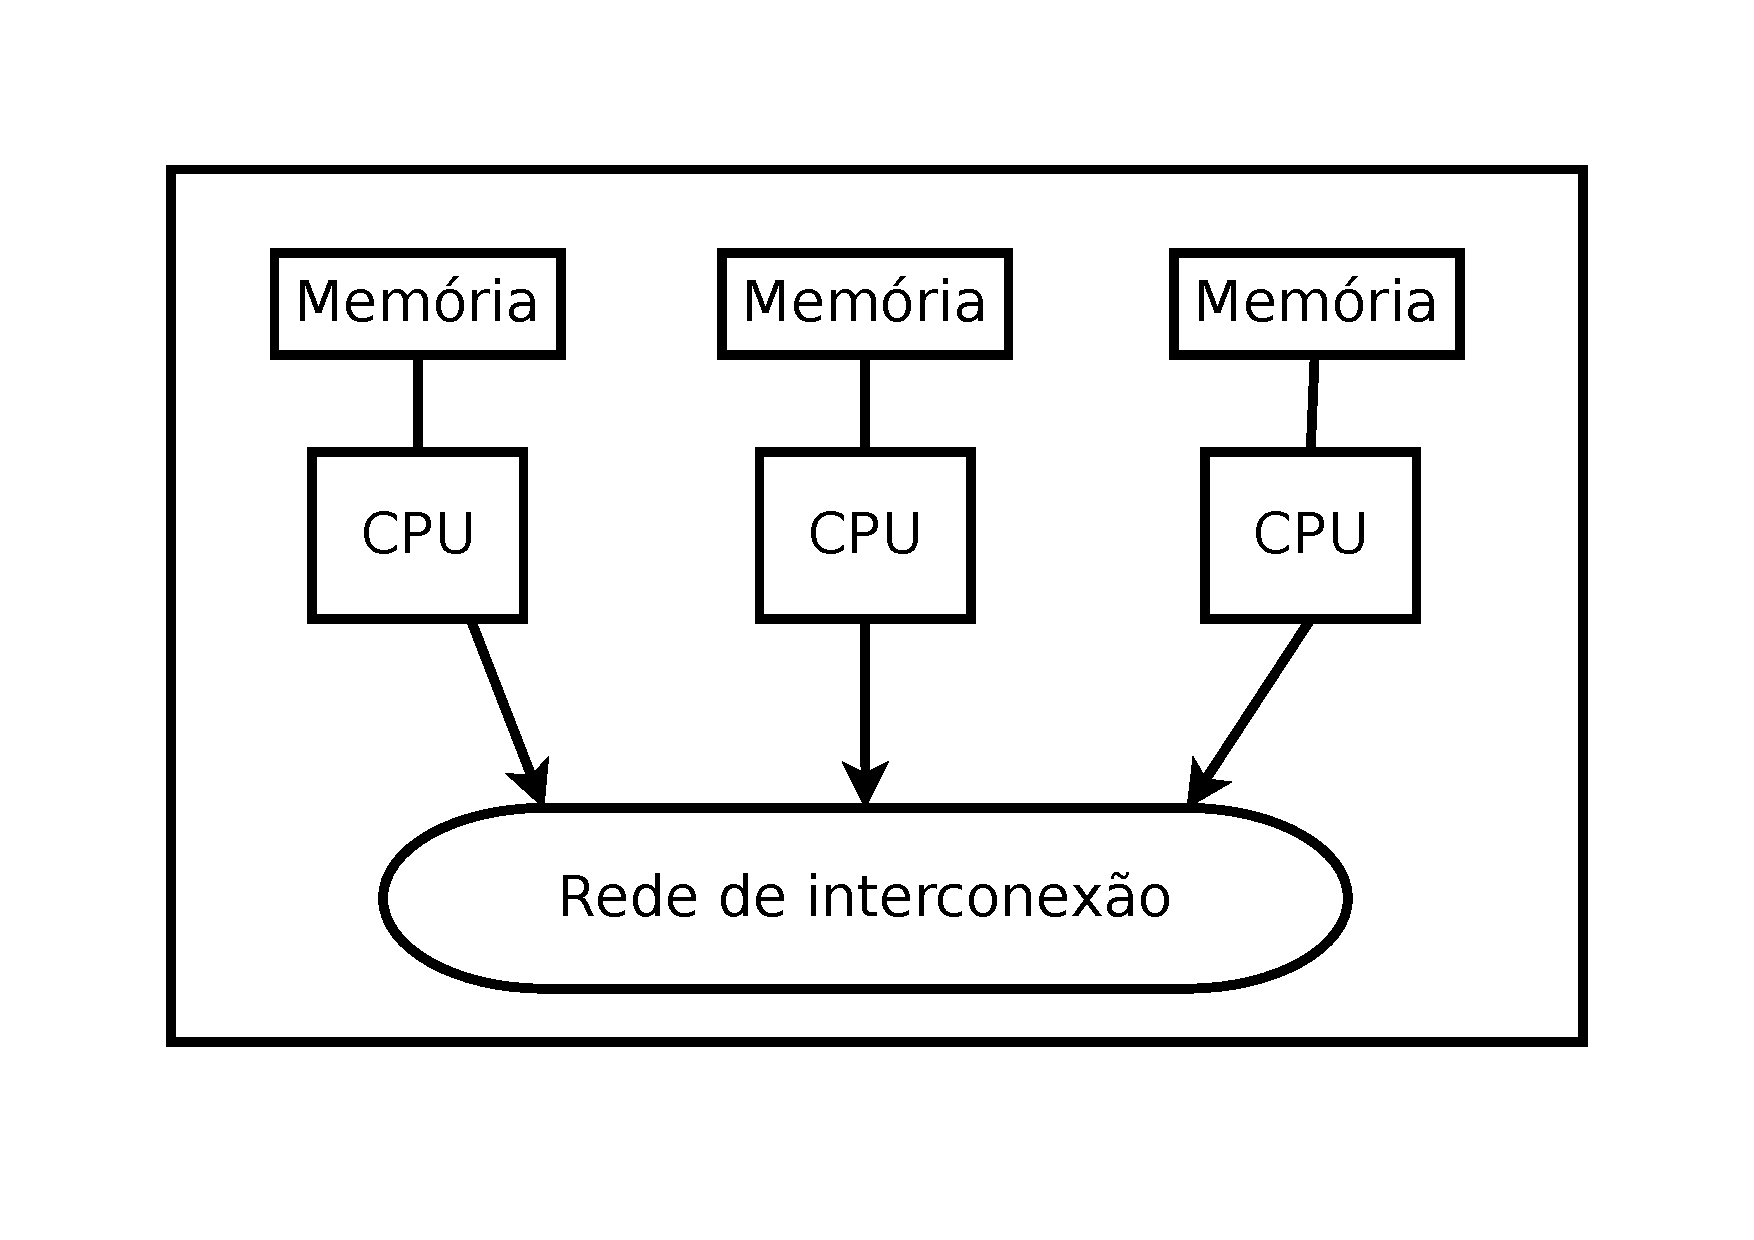
\includegraphics[trim=0cm 1cm 0cm 0cm, width=0.5\textwidth]{figuras/Arquitetura.pdf}
\caption{Modelo de programação por memória distribuída}
\label{fig:ArquiteturaDistribuida}
\end{figure}


\subsection{Computação paralela em \textit{clusters}}
Com o avanço tecnólogico da última década, o volume crescente de dados gerados, coletados e armazenados tornou o processamento dos dados inviável em um único computador.
A necessidade de manipular tais volumes de dados coloca em foco a computação de grandes volumes de dados, que requerem alto desempenho, em detrimento do modelo de processamento em supercomputadores.  Como resultado, torna-se crucial substituir a computação tradicional por computação distribuída eficiente, e é um caminho natural para o processamento de dados em larga escala o uso de \textit{clusters} ~\cite{Lin:2010}.

\textit{Clusters} são conjuntos de máquinas, ligadas em rede, que comunicam-se, trabalhando como se fossem uma única máquina de grande porte. 
Dentre algumas características observadas em um \textit{cluster}, é possível destacar: o baixo custo se comparado a supercomputadores; a proximidade geográfica dos nós; altas taxas de transferência nas conexões entre as máquinas e o uso de máquinas em geral homogêneas \cite{Toth:2008}.

Apesar dos computadores em um \textit{cluster} não precisarem processar necessariamente a mesma aplicação, a grande vantagem de tal organização é a habilidade de cada nó processar individualmente uma fração da aplicação, resultando em desempenho que pode ser comparado ao de um supercomputador.
Em geral os computadores de \textit{clusters} são de baixo custo, o que permite que um grande número de máquinas seja interligado, garantindo desempenho e melhor custo-benefício que os supercomputadores, o que apresenta outra vantagem. Além disso, novas máquinas podem ser facilmente incorporadas  ao \textit{cluster}, tornando-o uma solução mais flexível, principalmente por ser formado por máquinas de capacidade de processamento similar.

O bom desempenho das aplicações em \textit{clusters} envolve conceitos relacionados à infraestrutura, principalmente comunicação entre os nós e balanceamento de carga.
Para que o processamento do \textit{cluster} possa ser utilizado de maneira eficiente, é importante que os dados a serem processados sejam transferidos rapidamente pelas de redes de alta velocidade, para evitar que os processadores fiquem ociosos, subutilizando o poder de processamento do \textit{cluster}\cite{Rauber:2010}. 


\subsection{Computação paralela em grandes volumes de dados}
O processamento em \textit{clusters} é uma tarefa cujo desempenho é dependente de diversos fatores, como descrito anteriormente. O processamento de grandes volumes de dados também é uma tarefa desafiadora, que tem sido objeto de vários estudos. Os sistemas utilizados para processar grandes volumes de dados devem se basear em alguns princípios para garantir a escalabilidade e o bom desempenho.

A coleta e manutenção dos dados devem ser funções do sistema e não tarefa dos usuários. O sistema deve prover tratamento intrínseco dos dados  e os usuários devem ter facilidade para acessá-los. Mecanismos de confiabilidade, como replicação e  correção de erros devem ser incorporados como parte do sistema de modo a garantir integridade e disponibilidade dos dados.
O uso de modelos de programação paralela de alto nível também deve ser incentivado. O desenvolvedor deve utilizar programação de alto nível que não inclua configurações específicas de uma máquina. O trabalho de distribuir a computação entre as máquinas de forma eficiente deve ficar a cargo do sistema, e não do desenvolvedor.

%Os usuários devem ser capazes de executar programas de forma interativa, com variação dos requisitos de computação e armazenamento. O sistema deve responder rapidamente à consultas e cálculos simples, e não degradar o desempenho geral quando a tarefa for complexa. 
%Para suportar a computação interativa, deve haver oferta de recursos. O custo consequente do aumento dos recursos ofertados pode ser justificado com base no aumento da produtividade dos usuários do sistema.

Além disso, um sistema para computação de grandes volumes de dados deve implementar mecanismos de confiabilidade, no qual os dados originais e intermediários sejam armazenados de forma redundante. Isso permite que, no caso de falhas de componente ou dados, seja possível refazer a computação. Além disso, a máquina deve identificar e desativar automaticamente componentes que falharam, de modo a não prejudicar o desempenho do sistema e se manter sempre disponível \cite{Bryant:2011}.

Grandes empresas de serviços de Internet - como Google, Yahoo!, Facebook e Amazon - buscam soluções para processamento de dados em grandes conjuntos de máquinas que atendam as características descritas, pois com um software que possa prover tais características é possível alcançar alto grau de escalabilidade e custo-benefício. 

Dentre as principais propostas está o modelo MapReduce e sua implementação Hadoop, que são soluções escaláveis, capazes de processar grandes volumes de dados, com alto nível de abstração para distribuir a aplicação e mecanismos de tolerância a falhas.
A próxima seção apresenta com mais detalhes o modelo e suas características.

\section{MapReduce}
O MapReduce é um modelo de programação paralela criado pela Google para processamento de grandes volumes de dados em \textit{clusters}. Esse modelo propõe simplificar a computação paralela e ser de fácil uso, abstraindo conceitos complexos da paralelização - como tolerância a falhas, distribuição de dados e balanceamento de carga - e utilizando duas funções principais: Map e Reduce. Os princípios do desenvolvimento paralelo não são vistos pelo desenvolvedor, que pode se ocupar em desenvolver a solução proposta \cite{Dean:2008}.

Esse modelo de programação é inspirado em linguagens funcionais, tendo como base as primitivas Map e Reduce.
Os dados de entrada são específicos para cada aplicação e descritos pelo usuário.
A função Map é aplicada aos dados de entrada e produz uma lista intermediária de pares (chave, valor). Todos os valores intermediários associados a uma mesma chave são agrupados e enviados à função Reduce.
A função Reduce então
%aplicada a todos os pares intermediários com a mesma chave. A função
combina esses valores para formar um conjunto menor de resultados.
Tipicamente há apenas zero ou um valor de saída em cada função Reduce. Esses valores são agrupados na forma de pares no formato (chave, valor), que representam a saída da função.

Os Algoritmos \ref{funcaoMap} e \ref{funcaoReduce} apresentam um exemplo de uso do MapReduce, cujo objetivo é contar a quantidade de ocorrências de cada palavra em um documento. A função Map recebe como valor uma linha do documento, e como chave o número da linha. Para cada palavra encontrada na linha recebida, a função emite a palavra e a contagem de uma ocorrência. A função Reduce recebe como chave uma palavra e uma lista dos valores emitidos pela função Map, associados à palavra em questão. As ocorrências da palavra são agrupadas e a função retorna a palavra e seu total de ocorrências.

%\begin{lstlisting}[label=some-code,caption=Pseudocódigo para contagem de palavras no modelo MapReduce]
%Function Map (Integer chave, String valor):
%	#chave: número da linha no arquivo.
%	#valor: texto da linha correspondente.
%	listaDePalavras = split (valor)
%	for palavra in listaDePalavras:
%		emit (palavra, 1)
%Function Reduce (String chave, Iterator valores):
%	#chave: palavra emitida pela função Map.
%	#valores: conjunto de valores emitidos para a chave.
%	total = 0
%	for v in valores:
%		total = total + 1
%	emit (palavra, total)
%\end{lstlisting}

\SetAlCapSkip{0.6cm}

\begin{algorithm}	
\DontPrintSemicolon
	\SetKw{In}{in}
	\SetKwFunction{Emit}{Emit}
	\SetKwFunction{Split}{Split}
  	\SetKwBlock{Begin}{Function Map(Integer chave, String valor)}{end}
  	\Begin{
		\BlankLine
		\emph{chave: número da linha no arquivo \\
				valor: texto da linha correspondente}
		\BlankLine
		listaDePalavras $\leftarrow$ \Split(valor)\;
		\BlankLine
		\ForEach{palavra \In listaDePalavras}{
	    		\Emit(palavra, 1)\;
		}
	}
	\caption{Função Map (Integer chave, String valor)}\label{funcaoMap}
\end{algorithm}

\begin{algorithm}	 
\DontPrintSemicolon
	\SetKw{In}{in}
	\SetKwFunction{Emit}{Emit}
	\SetKwBlock{Begin}{Function Reduce (String chave, Iterator valores)}{end}
	\Begin{
		\BlankLine
		\emph{chave: palavra emitida pela função Map \\
			valores: conjunto de valores emitidos para a chave}
		\BlankLine
		total $\leftarrow 0$\;
		\BlankLine
		\ForEach{v \In valores}{
			total $\leftarrow$ total + 1\;
	    }
	    	\Emit(palavra, total)
    }
	\caption{Função Reduce (String chave, Iterator valores)}\label{funcaoReduce}
\end{algorithm}


A Figura \ref{fig:MapReduceexemplo} ilustra o fluxo de execução para este exemplo. A entrada é um arquivo contendo as linhas ``hadoop conta'', ``conta palavras'' e ``exemplo hadoop''.

\begin{figure}[!h]
\centering
%trim left, bottom, right and top
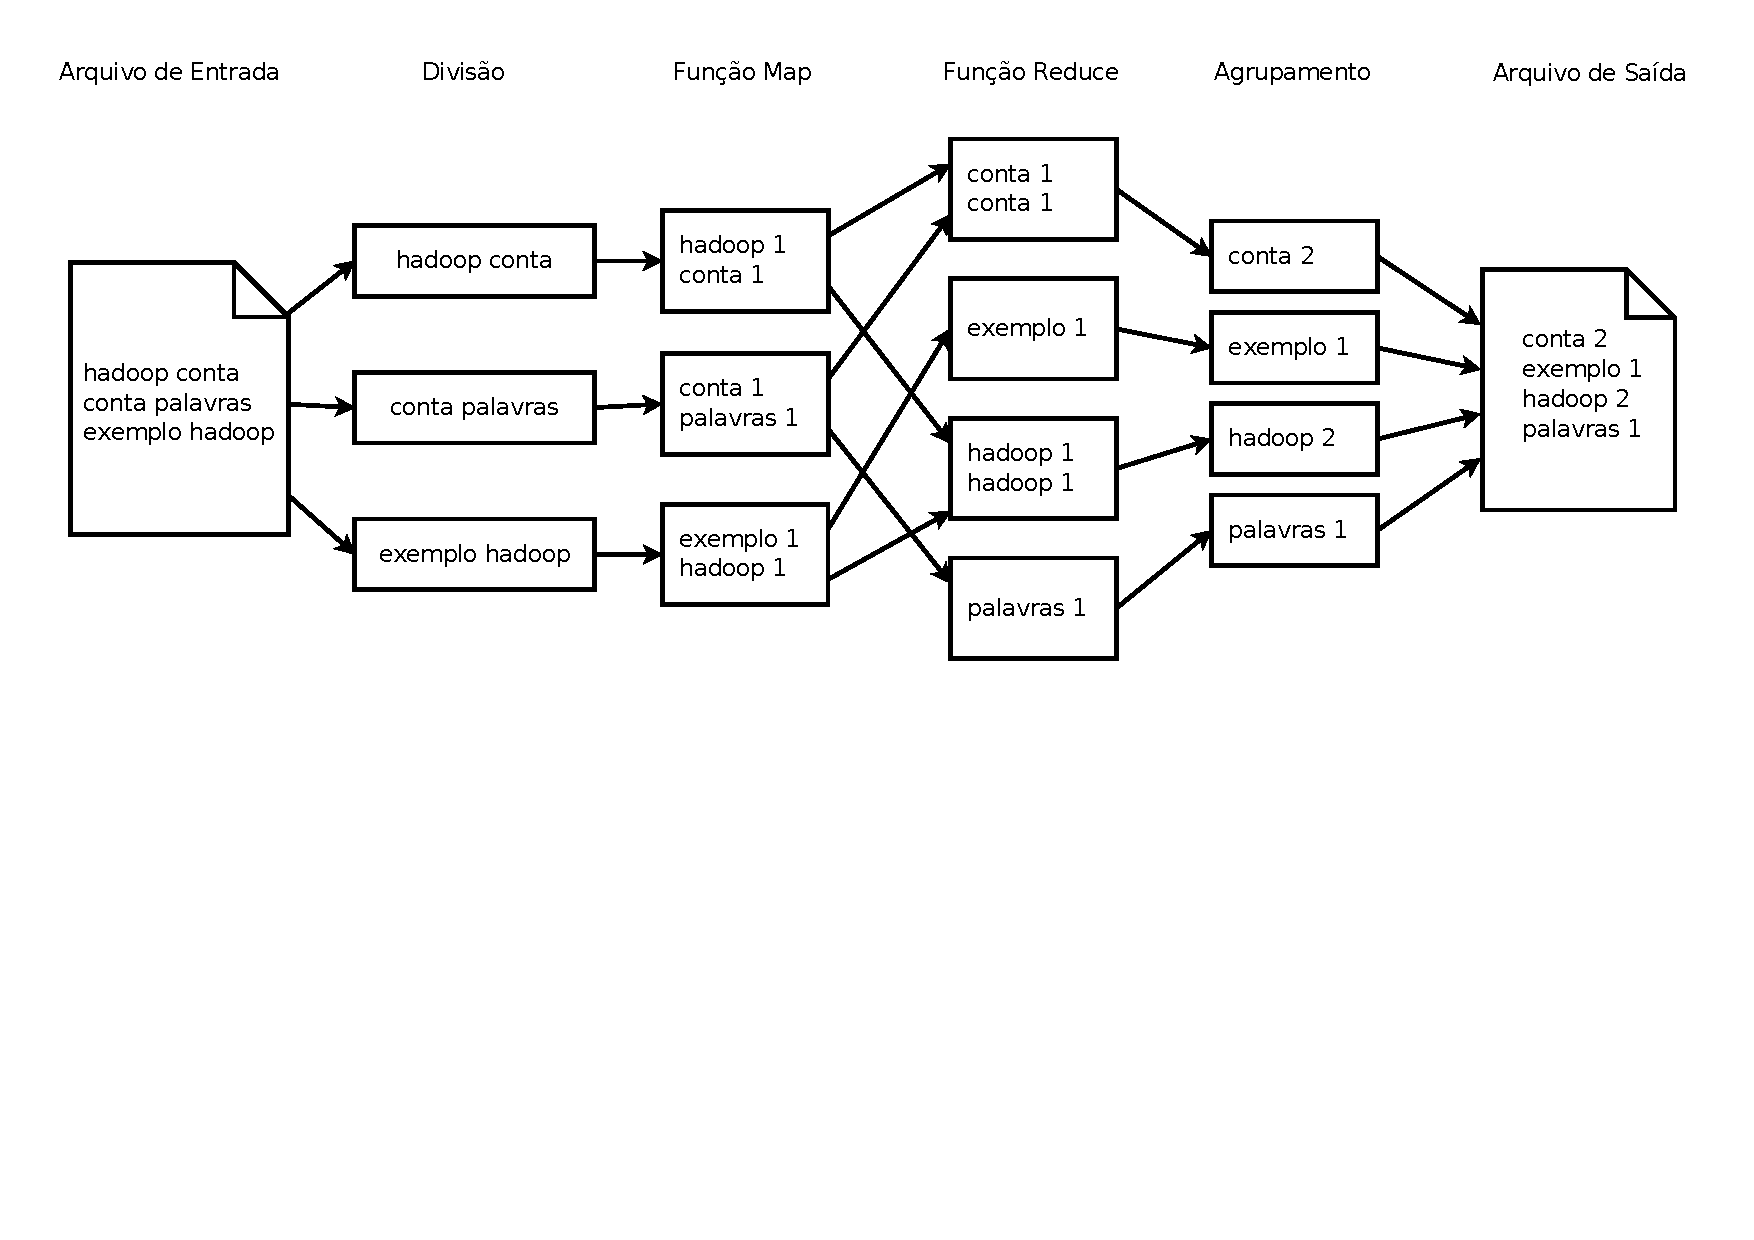
\includegraphics[trim=0cm 9cm 0cm 0cm, width=\textwidth]{figuras/MapReduceExemplo.pdf}
\caption{Exemplo da contagem de palavras com o MapReduce}
\label{fig:MapReduceexemplo}
\end{figure}

\subsection{Arquitetura do MapReduce}
O MapReduce é constituído de uma arquitetura do tipo mestre-escravo com dois tipos principais de nós: \textit{Master} e \textit{Worker}. O nó mestre tem como função atender requisições de execução dos usuários, gerenciá-las, criar tarefas e distribuí-las entre os nós trabalhadores, que executam as tarefas com base nas funções Map e Reduce definidas pelo usuário.
%Como é possível perceber, trata-se de uma típica arquitetura mestre-escravo (do inglês master-slave) (DUBREUIL; GAGNÉ; PARIZEAU, 2006).
A arquitetura também inclui um sistema de arquivos distribuídos, onde ficam armazenados os dados de entrada e intermediários.
%Para evitar a transferência excessiva de dados, os \textit{workers} do MapReduce são também nós do sistema de arquivos.


% }

\subsection{Visão geral do fluxo de execução}


As chamadas da função Map são distribuídas automaticamente entre as diversas máquinas através do particionamento dos dados de entrada em \textit{M} conjuntos. Cada conjunto pode ser processado em paralelo por diferentes máquinas. As chamadas da função Reduce são distribuídas pelo particionamento do conjunto intermediário de pares em \textit{R} partes. O número de partições \textit{R} pode ser definido pelo usuário.

A Figura \ref{fig:MapReduceoverview} ilustra o fluxo de uma execução do modelo MapReduce \cite{Dean:2008}. A sequência de ações descrita a seguir explica o que ocorre em cada um dos passos. A numeração dos itens a seguir corresponde à numeração da figura.

 \begin{figure}[!htb]
 \centering
%trim left, bottom, right and top
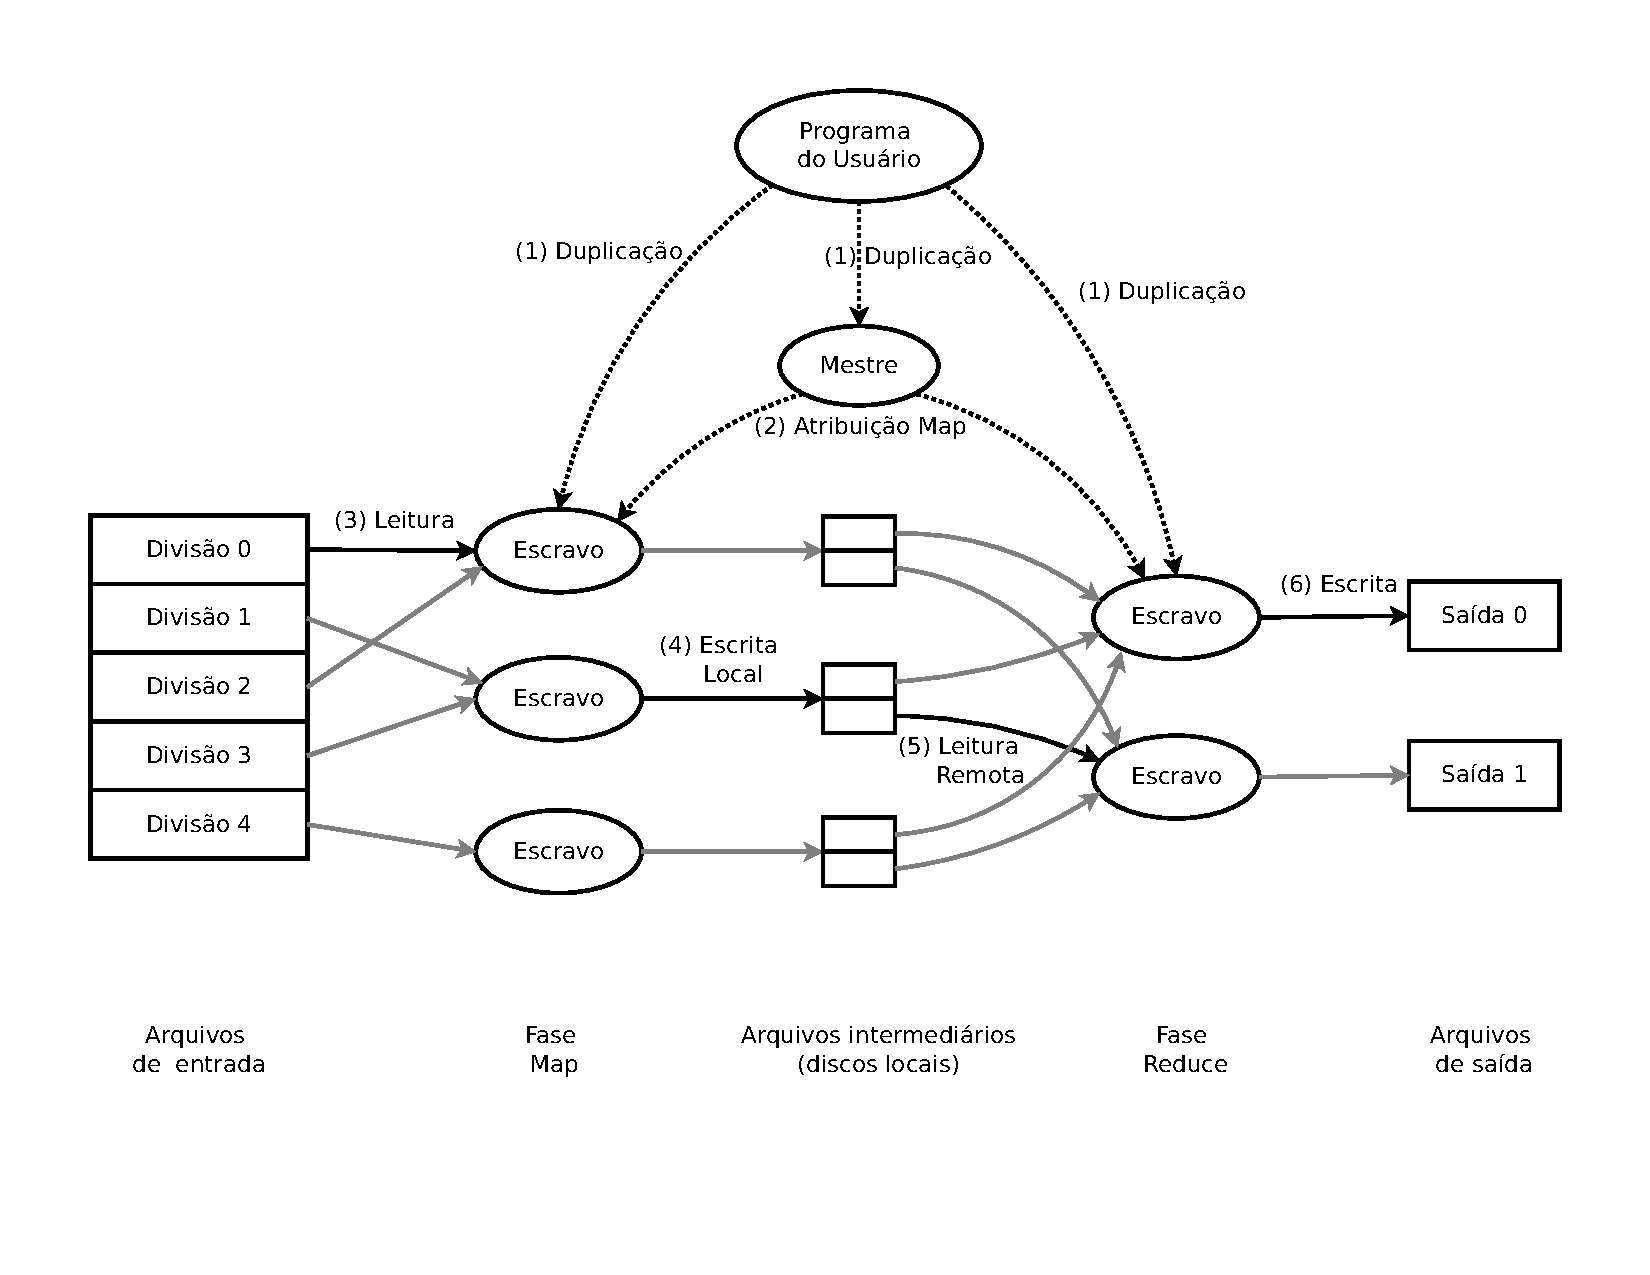
\includegraphics[trim=0cm 2cm 0cm 1cm, width=\textwidth]{figuras/MapReduceOverflow.pdf}
\caption{Visão geral do funcionamento do modelo MapReduce}
\label{fig:MapReduceoverview}
\end{figure}

\begin{enumerate}
\item A biblioteca MapReduce, no programa do usuário, divide os arquivos de entrada em M pedaços. Em seguida, iniciam-se muitas cópias do programa para o conjunto de máquinas;

\item Uma das cópias do programa é especial: o mestre (\textit{Master}). Os demais são trabalhadores (\textit{Workers}) cujo trabalho é atribuído pelo mestre. Existem M tarefas Map e R tarefas Reduce a serem atribuídas. O mestre atribui aos trabalhadores ociosos uma tarefa Map ou uma tarefa Reduce;

\item Um trabalhador que recebe uma tarefa Map lê o conteúdo do fragmento de entrada correspondente. Ele cria pares (chave, valor) a partir dos dados de entrada e encaminha cada par para a função Map definida pelo usuário. Os pares (chave, valor) intermediários, produzidos pela função Map, são colocados no \textit{buffer} de memória;

\item Periodicamente, os pares colocados no \textit{buffer} são gravados no disco local, divididos em R regiões  pela função de particionamento. As localizações desses pares bufferizados, no disco local, são passadas de volta para o mestre que é responsável pelo encaminhamento desses locais aos trabalhadores Reduce;

\item Quando um trabalhador Reduce é notificado pelo mestre sobre essas localizações, ele usa chamadas de procedimento remoto para ler os dados dos discos locais dos trabalhadores Map. Quando um trabalhador Reduce tiver lido todos os dados intermediários da sua partição, ele a ordena pelas chaves intermediárias, de forma que todas as ocorrências da mesma chave estejam agrupadas. Se a quantidade de dados intermediários é muito grande para caber na memória, um tipo de ordenação externa é usado;

\item O trabalhador Reduce itera sobre os dados intermediários ordenados e, para cada chave encontrada, repassa a chave e o conjunto correspondente de valores intermediários para função Reduce do usuário. A saída da função Reduce é anexada a um arquivo de saída final para essa partição Reduce;

             	        	
\end{enumerate}

Após todas as tarefas Map e Reduce concluídas, o mestre acorda o programa do usuário, retornando, neste ponto, a chamada MapReduce para o código do usuário.

\section{Hadoop}

O Hadoop é uma das  implementações mais conhecidas do modelo MapReduce. Ele provê o gerenciamento de computação distribuída, de maneira escalável e confiável. É uma implementação código aberto em Java  desenvolvida por Doug Cutting em 2005 e mantida pela Apache Software Foundation \cite{White:2009, Hadoop:2010}.

Um dos principais benefícios do Hadoop é permitir o processamento em conjunto de centenas de máquinas de maneira transparente, o que significa que o usuário não deve se preocupar com mecanismos de tolerância a falhas, que são providos pelo sistema. %\cite{Dean:2008}. 
Facebook, Yahoo! e eBay utilizam o ambiente Hadoop em seus \textit{clusters}, para processar diariamente terabytes de dados e logs de eventos para detecção de \textit{spam}, \textit{business intelligence} e diferentes tipos de otimização \cite{Cherkasova:2011}.

O mecanismo de tolerância a falhas implementado pelo sistema permite que o trabalho do usuário possa ser concluído mesmo que ocorra alguma falha de disco, de processo ou de nó. Periodicamente, o nó mestre envia mensagens aos demais nós para verificar seus estados. Se nenhuma resposta é recebida, o mestre identifica que houve falha neste nó e o substitui. 
As tarefas que não foram executadas são reescalonadas para os demais nós. O mecanismo de replicação garante que sempre haja um número determinado de cópias dos dados, e caso um dos nós de armazenamento seja perdido, os demais se encarregam de realizar uma nova replicação \cite{White:2009}.
 % O sistema é capaz de verificar e substituir nós quando ocorre alguma falha. 

\subsection{Arquitetura do \textit{framework}}

A arquitetura do Hadoop é baseada nos conceitos da arquitetura do MapReduce e, portanto, também é do tipo mestre-escravo. No Hadoop são definidos nós mestres e escravos tanto para a execução de tarefas quanto para o sistema de arquivos.
O nó mestre consiste em um \textit{JobTracker}  para as tarefas MapReduce e um \textit{NameNode}  responsável por manter e controlar todos os metadados do sistema de arquivos e gerenciar a localização dos dados. O nó mestre também é responsável por outras atividades como, por exemplo, balanceamento de carga, \textit{garbage collection} e atendimento a requisições dos clientes.
Os nós escravos são formados por um \textit{TaskTracker}  para as tarefas MapReduce e por um \textit{DataNode} responsável por armazenar e transmitir os dados aos usuários que os requisitarem.

A Figura \ref{fig:hdfs} apresenta a formação de um \textit{cluster} típico, ilustrando a arquitetura do \textit{framework}, incluindo o sistema de arquivos distribuídos.
O \textit{NameNode} gerencia e manipula todas as informações dos arquivos, tal como a localização e o acesso. Os \textit{DataNodes} se encarregam da leitura e escrita das informações nos sistemas de arquivo cliente. Os \textit{JobTracker} e \textit{TaskTracker} são responsáveis por executar as tarefas MapReduce.
\begin{figure}[htb]
\centering
%trim left, bottom, right and top
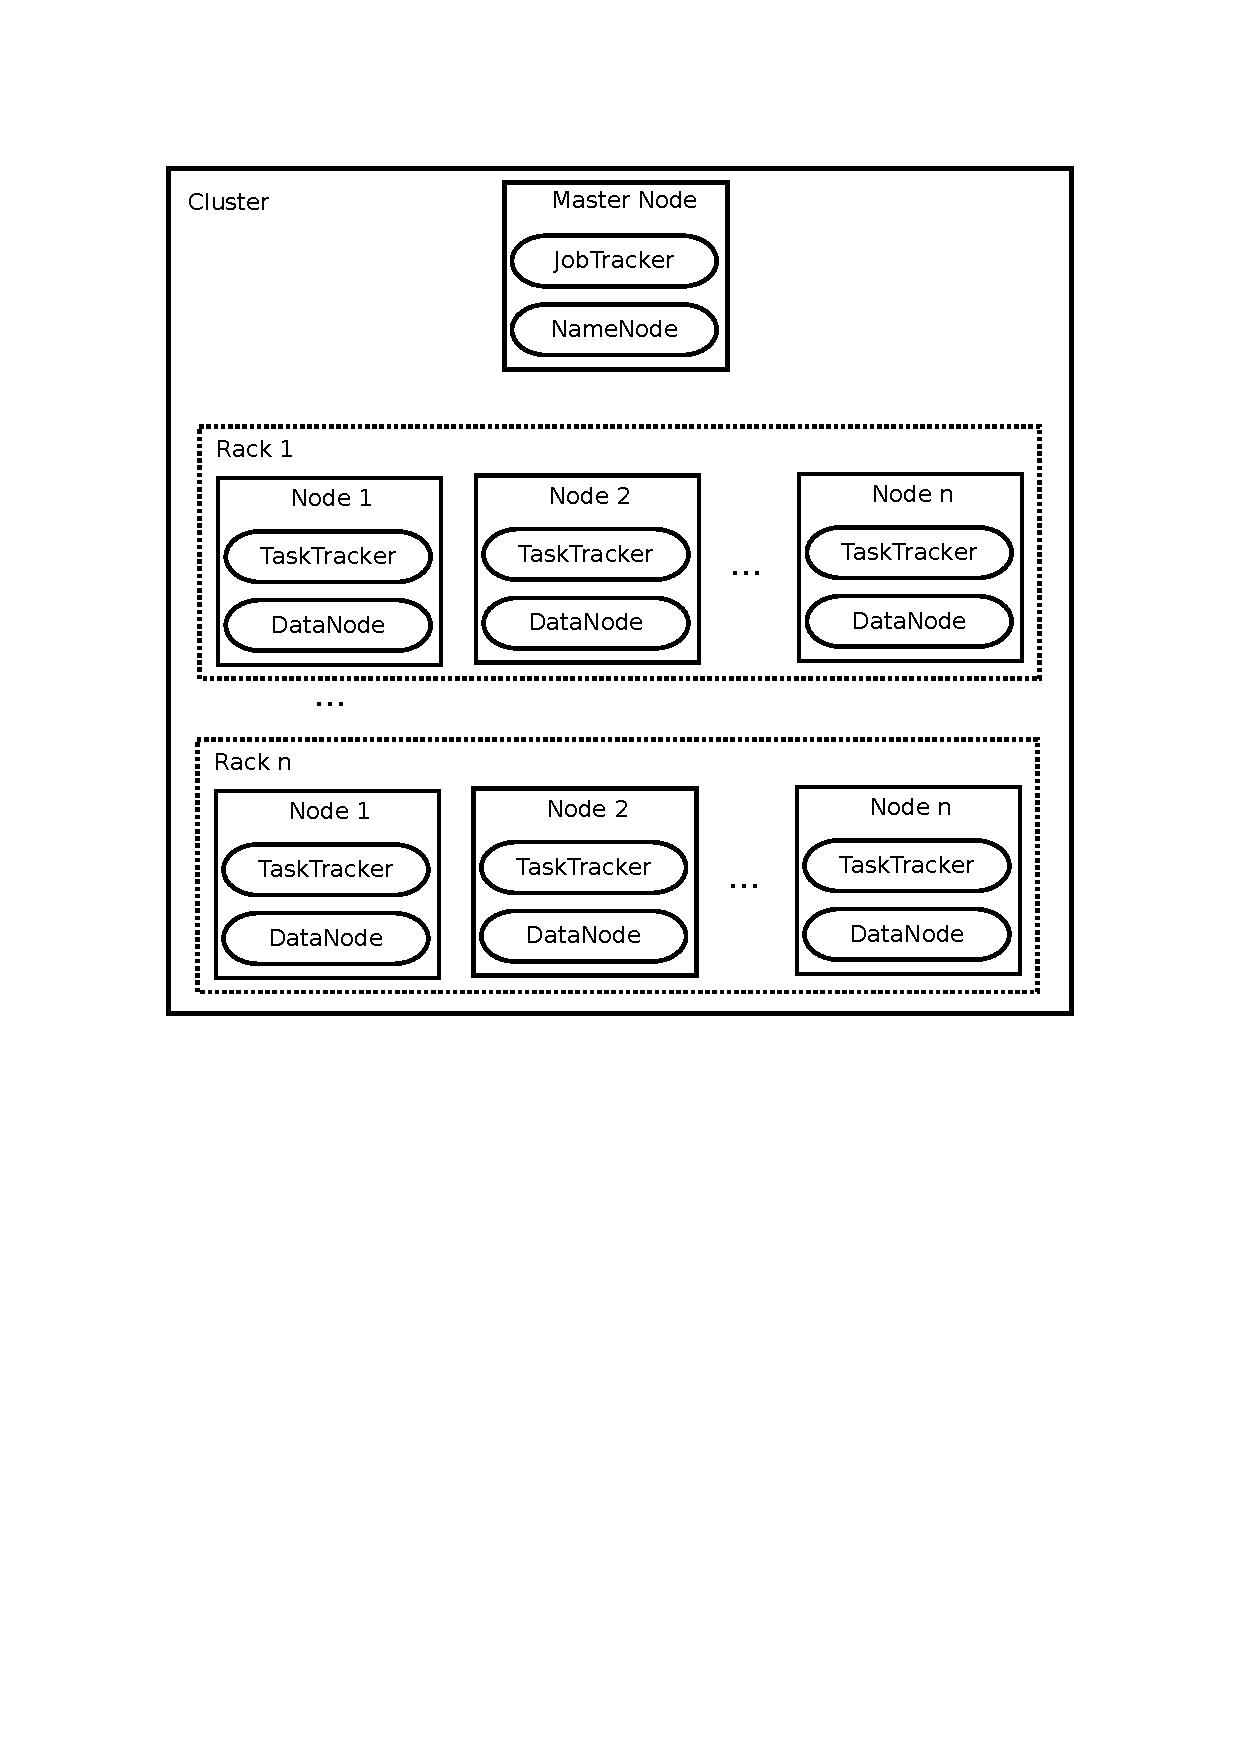
\includegraphics[trim=2cm 12cm 2cm 2cm, width=0.6\textwidth]{figuras/HadoopCluster.pdf}
\caption{Visão abstrata de um cluster típico. Baseado em \cite{Venner:2009}}
\label{fig:hdfs}
\end{figure}

\subsection{Sistema de Arquivos do Hadoop}

O \textit{ Hadoop Distributed File System} (HDFS) é um sistema de arquivos distribuído desenvolvido para armazenar grandes conjuntos de dados e ser altamente tolerante a falhas \cite{White:2009}.
A plataforma Hadoop fornece o HDSF como sistema de arquivos padrão, mas é compatível com diversos sistemas de arquivos distintos, como Amazon S3 (Native e Block-based), CloudStore, HAR, Local (destinado a unidades de armazenamento conectadas localmente) e sistemas mantidos por servidores FTP e HTTP.

O HDFS incorpora funcionalidades que têm grande impacto no desempenho geral do sistema.
Uma delas é conhecida como \textit{rack awareness}. Com esse recurso, o sistema de arquivos é capaz de identificar os nós escravos que pertencem a um mesmo \textit{rack}, e distribuir as réplicas de maneira a melhorar o desempenho e a confiabilidade do sistema.
Outra funcionalidade é a distribuição das tarefas considerando localização dos dados nos nós. O sistema de arquivos procura manter um balanceamento na ocupação das unidades de armazenamento, e o \textit{framework} busca atribuir tarefas a um escravo que possua, em sua unidade de armazenamento local, os dados que devem ser processados.
Assim, quando executa-se grandes operações MapReduce com um número significativo de nós, a maioria dos dados são lidos localmente e o consumo de banda é mínimo.